\documentclass[11pt]{article}
\usepackage[T1]{fontenc}
\usepackage[utf8]{inputenc}
\usepackage{lmodern}
\usepackage[margin=1in]{geometry}
\usepackage{amsmath,amssymb}
\usepackage{booktabs}
\usepackage{multirow}
\usepackage{tikz}
\usetikzlibrary{positioning,arrows.meta,fit,backgrounds}
\usepackage{graphicx}
\usepackage{xcolor}
\usepackage{microtype}
\usepackage[hidelinks]{hyperref}
\usepackage[numbers,sort&compress]{natbib}

\newcommand{\dee}{\textsc{DEE}}
\newcommand{\killed}{\textbf{KILLED}}

\title{Exact by Construction, Graded in Advance:\\
A Pre-Registered Hardware Evaluation of SSD-to-GPU\\
Expert Offloading for DeepSeek-V4-Flash}

\author{Nivin Karthick \\ Independent researcher \\
\texttt{\small https://github.com/so-nerdyy/dee}}

\date{November 2026}

\begin{document}
\maketitle

\begin{abstract}
Mixture-of-experts (MoE) models can run on GPUs far smaller than the model by
keeping most expert weights on SSD or in host RAM and loading them on demand.
Recent offloading systems report large speedups, but they rarely check that the
offloaded model produces the same tokens as the unoffloaded one, and their
performance numbers are not tested against predictions made before the
experiment. We describe \dee{} (Dynamic Expert Eviction), an engine that serves
DeepSeek-V4-Flash (43 MoE layers, 256 routed experts per layer, a 146.6\,GiB
FP4 expert store) from an NVMe-backed two-tier cache, and we evaluate it in a
way that is designed to be falsifiable. First, \dee{} enforces an
\emph{exactness contract}: caching, placement and scheduling may change, but the
generated token ids and the full per-layer routing journal must be
byte-identical to a reference run. Second, before any cloud GPU run existed, we
froze a prediction matrix (decode tokens/s, host-cache hit rate, cold reads per
token and cost) with kill bands, and graded every later run against it.
Across seven runs on six Modal GPU configurations (under \$14 of compute in
total), every run met the exactness contract on its own hardware, and a 2$\times$T4
container reproduced a reference answer sealed three months earlier on different
infrastructure token for token. Most of our pre-registered throughput
predictions were wrong: 9 of 12 testable decode-speed rows were killed, with
measured speed 2--6.5$\times$ below the registered nominal. Two negative results
came out of the same discipline: learned and heuristic expert prefetch hints did
not pay for their extra reads, offline or on hardware. One positive result held
exactly as registered: replacing LRU with a next-use eviction rule removed a
0\% host-hit cliff at batch size 8 and raised throughput 1.30$\times$ (predicted
1.27$\times$). The fastest configuration, an RTX PRO 6000, decoded 6.27
tokens/s in aggregate at batch 8; on rented GPUs that costs far more per token
than hosted APIs, so the case for offloading is running a model larger than
the GPU's memory, verifiably, not serving it cheaply. We release the engine, the frozen
predictions, all scorecards and the scorer.
\end{abstract}

\section{Introduction}

Sparse mixture-of-experts language models activate only a few experts per token
\citep{shazeer2017outrageously,lepikhin2021gshard,fedus2022switch,dai2024deepseekmoe}.
DeepSeek-V4-Flash, the model we study, routes each token to 6 of 256 experts in
each of 43 layers, plus one shared expert \citep{dsv4flash}. Most of the model's
bytes are routed-expert weights that any given token never touches, which makes
it natural to keep those weights on slower storage and fetch them on demand. A
line of systems does exactly this, from host-RAM offloading
\citep{eliseev2023mixtral,xue2024moeinfinity,kamahori2024fiddler,cao2024moelightning}
to SSD-backed and edge designs
\citep{yi2023edgemoe,alizadeh2024llminaflash,song2024powerinfer},
with expert-activation predictors used to prefetch weights before they are
needed \citep{hwang2024pregated,song2024promoe,he2024expertflow,wang2026seqmoe}.

These papers mostly report speed. Two things are usually missing. The first is a
check that offloading did not change the model's output. Offloading code touches
expert selection, ordering and numerics, and an approximation or a bug in any of
them can change tokens while leaving the speed numbers looking good. Some
systems change routing on purpose (for example by substituting a resident
expert for a missing one), which is a legitimate design choice but means the
served model is no longer the published one. The second is a test of the
performance claims against predictions made in advance. Without one, a cost
model fitted after the fact will always look accurate.

\dee{} is a small, single-author research engine, and it is slower than the
fastest recent systems on similar hardware (Section~\ref{sec:related}). This
paper does not argue that it is the fastest, and it does not argue that
offloading is a cheaper way to serve a model: on rented GPUs it costs orders of
magnitude more per token than hosted APIs (Section~\ref{sec:limits}). What
offloading buys is the ability to run a model whose weights do not fit in GPU
memory on a GPU you already have. This paper reports what happens when such an
engine is held to two rules:

\begin{enumerate}
\item \textbf{Exactness.} Placement may change; outputs may not. Every run
records the generated token ids and a chain-hashed journal of every routed
expert in every layer for every forward step, and these must be byte-identical
to a reference run (Section~\ref{sec:exact}).
\item \textbf{Pre-registration.} A prediction matrix for the cloud campaign was
committed to git on 2026-09-30, when no cloud GPU run existed. Each cell has a
nominal value, a working range and a kill band. Later information can only be
appended as dated addenda; frozen ranges are never edited
(Section~\ref{sec:prereg}). Pre-registration is standard in other empirical
sciences \citep{nosek2018preregistration} and has recently been used for an MoE
caching study \citep{suram2026cacheable}.
\end{enumerate}

Our contributions are:
\begin{itemize}
\item An engine that serves DeepSeek-V4-Flash from a 146.6\,GiB segmented FP4
expert store through a VRAM cache and a pinned host-RAM cache, with an
end-to-end exactness gate on tokens and routing journals (Sections~\ref{sec:system}--\ref{sec:exact}).
\item A pre-registered evaluation on six Modal GPU configurations (T4, A10, L4,
L40S, RTX PRO 6000; one and two GPUs), graded against frozen bands and
reported in full, including the rows that were killed (Section~\ref{sec:results}).
\item Evidence that exactness is reproducible across infrastructure: a run on
Modal 2$\times$T4 in November 2026 reproduced the reference answer sealed on
Kaggle 2$\times$T4 in August 2026, while different GPU architectures
produce different (self-consistent) tokens, which we attribute to
floating-point drift at near-tie router decisions (Section~\ref{sec:crossgpu}).
\item Two documented negative results on prefetching and one confirmed positive
result on eviction, each with its prediction, its measurement and the cause of
any miss (Section~\ref{sec:policy}).
\end{itemize}

\section{Background and related work}\label{sec:related}

\paragraph{MoE offloading.}
Eliseev and Mazur \citep{eliseev2023mixtral} ran Mixtral-8x7B on consumer GPUs
with an LRU expert cache and speculative loading. MoE-Infinity
\citep{xue2024moeinfinity} traces activations per request to guide prefetching
and caching. Fiddler \citep{kamahori2024fiddler} and MoE-Lightning
\citep{cao2024moelightning} use the CPU to compute experts instead of moving
them. EdgeMoE \citep{yi2023edgemoe} targets mobile devices; LLM in a Flash
\citep{alizadeh2024llminaflash} and PowerInfer \citep{song2024powerinfer} exploit
activation sparsity to serve dense models from flash or CPU memory. FlexGen
\citep{sheng2023flexgen} schedules offloading for throughput-oriented batch
inference. DALI \citep{zhu2026dali} assigns experts between CPU and GPU by
workload. SpecMD \citep{hoang2026specmd} benchmarks caching and prefetching
policies under controlled bandwidth and proposes a Least-Stale eviction rule.

\paragraph{Expert prediction and prefetching.}
Pre-gated MoE \citep{hwang2024pregated} changes the architecture so that the
router for the next layer runs one layer early. ProMoE \citep{song2024promoe} and
ExpertFlow \citep{he2024expertflow} learn or adapt predictors of upcoming expert
use. SeqMoE \citep{wang2026seqmoe} treats expert prediction as sequence modeling
with a Mamba2 predictor, schedules prefetches by deadline, evicts by predicted
next use (``probabilistic Belady''), and evaluates on DeepSeek-V4-Flash among
other models. Our next-use eviction rule and deadline-ordered queue follow
SeqMoE's ideas; the offline bound we compare against is Belady's MIN
\citep{belady1966study}.

\paragraph{Systems on the same model.}
At least two recent systems serve DeepSeek-V4-Flash under memory limits. SeqMoE
reports results on an RTX PRO 6000 Blackwell (96\,GB) \citep{wang2026seqmoe};
MoE-CORE runs a W4A8 version on an Ascend NPU under an 84\,GB device-memory cap
\citep{yang2026moecore}. Both keep the offloaded weights in host DRAM rather than
on SSD. SeqMoE reports reaching a large fraction of full-load performance, well
above what \dee{} achieves. As far as we can tell, neither gates on
byte-identical tokens and routing against an unoffloaded reference. MoE-CORE
includes an optional score-based expert substitution path, which by design
changes routing. We have not run these systems ourselves, so we make no
head-to-head speed claim.

\paragraph{Pre-registration and reproducibility.}
Suram \citep{suram2026cacheable} pre-registered a training intervention for
cache-friendly routers and reported a negative result, alongside a systems
measurement of SSD-backed serving on a consumer GPU. Our use is narrower: we
pre-register the \emph{performance and cache predictions} of an inference
engine on specific cloud hardware. Run-to-run and cross-hardware
non-determinism in LLM inference is a known problem
\citep{yuan2025fp32}; our cross-GPU results (Section~\ref{sec:crossgpu}) are one
more data point.

\section{System}\label{sec:system}

\begin{figure}[htbp]
\centering
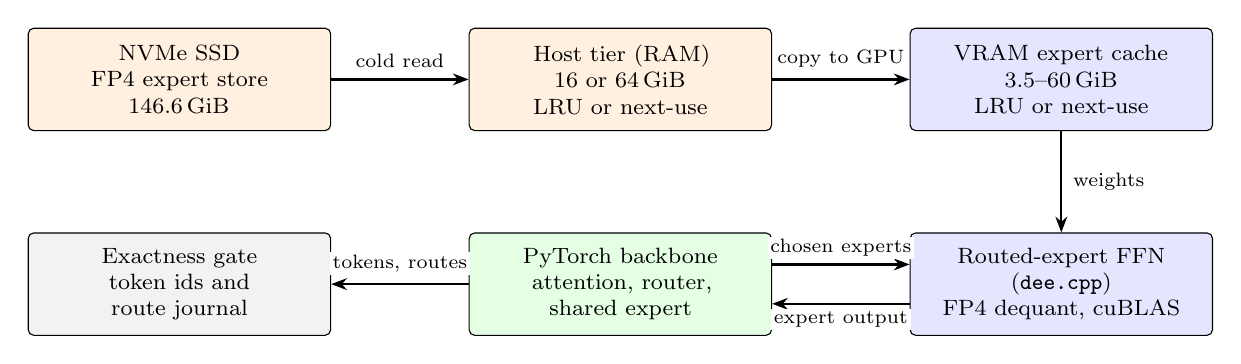
\begin{tikzpicture}[
  box/.style={draw, rounded corners=2pt, align=center, font=\footnotesize,
              minimum height=13mm, text width=37mm, inner sep=2pt},
  arr/.style={-{Stealth[length=2mm]}, thick},
  lab/.style={font=\scriptsize, align=center, fill=white, inner sep=1pt}]
\node[box, fill=orange!12] (ssd)  at (0,0)    {NVMe SSD\\FP4 expert store\\146.6\,GiB};
\node[box, fill=orange!12] (host) at (5.6,0)  {Host tier (RAM)\\16 or 64\,GiB\\LRU or next-use};
\node[box, fill=blue!10]   (vram) at (11.2,0) {VRAM expert cache\\3.5--60\,GiB\\LRU or next-use};
\node[box, fill=gray!10]   (gate) at (0,-2.6)    {Exactness gate\\token ids and\\route journal};
\node[box, fill=green!10]  (torch) at (5.6,-2.6) {PyTorch backbone\\attention, router,\\shared expert};
\node[box, fill=blue!10]   (ffn) at (11.2,-2.6)  {Routed-expert FFN\\(\texttt{dee.cpp})\\FP4 dequant, cuBLAS};
\draw[arr] (ssd) -- node[lab, above=1mm]{cold read} (host);
\draw[arr] (host) -- node[lab, above=1mm]{copy to GPU} (vram);
\draw[arr] (vram) -- node[lab, right=1mm]{weights} (ffn);
\draw[arr] ([yshift=2.5mm]torch.east) -- node[lab, above=0.5mm]{chosen experts} ([yshift=2.5mm]ffn.west);
\draw[arr] ([yshift=-2.5mm]ffn.west) -- node[lab, below=0.5mm]{expert output} ([yshift=-2.5mm]torch.east);
\draw[arr] (torch) -- node[lab, above=1mm]{tokens, routes} (gate);
\end{tikzpicture}
\caption{\dee{}'s data path. The router in the PyTorch backbone chooses
experts; the native engine only makes sure the chosen experts are on the GPU
(VRAM, else host tier, else SSD) and runs them. Placement policies act only on the
cache tiers (top row), never on the router. Every run's tokens and
routing journal go to the exactness gate.}
\label{fig:arch}
\end{figure}

Figure~\ref{fig:arch} shows the data path.

\paragraph{Model.} DeepSeek-V4-Flash-0731 (revision \texttt{9e165c30}) has 43
MoE layers with 256 routed experts each (top-6, \texttt{sqrtsoftplus} scores,
route scale 1.5), one shared expert per layer, hidden size 4096 and expert
intermediate size 2048 \citep{dsv4flash}. The first three layers are
hash-routed. Routed experts are stored in FP4 with block scales.

\paragraph{Split of work.} Tokenizer, attention, KV cache, router, shared expert,
normalization and LM head run in PyTorch (2.10.0+cu128, pinned) on a resident
backbone of about 8.2\,GiB. Routed experts run in a native C++/CUDA engine
(\texttt{dee.cpp}, exposed to Python as \texttt{pydee}): it receives the router's
selected experts and weights, makes sure the experts are on the GPU, dequantizes
FP4 on the GPU, and runs the SwiGLU FFN with cuBLAS. The engine never chooses
experts. The router's selection is always what executes.

\paragraph{Expert store.} The 11,776 expert records (43 layers $\times$ 256
experts, plus three MTP buckets) are packed into a segmented store of 46
segments, 13,369,344 bytes (12.75\,MiB) per record, 146.6\,GiB in total.
Every segment is checked against a SHA-256 table at staging time, and the
engine reports a store-integrity identity in every run.

\paragraph{Two-tier cache.} A request for (layer, expert) is served from a VRAM
expert cache if resident; otherwise from a pinned host-RAM cache
(\emph{host tier}); otherwise read from the store with \texttt{pread} on
several read lanes (a \emph{cold read}). The VRAM budget was 3,584\,MiB per GPU
on 24\,GB cards, 26,624\,MiB on the L40S and 61,440\,MiB on the RTX PRO 6000. The
host tier was 16 or 64\,GiB.

\paragraph{Eviction.} The baseline policy on both tiers is LRU. The
\emph{next-use} policy evicts the record whose expected next use is furthest away,
\begin{equation}
E = d + N\left(\frac{1}{p} - 1\right),
\end{equation}
where $d$ is the number of layer calls until the layer sweep returns to the
record's layer, $N=43$ is the number of layers, and $p$ is a running estimate of
how often the record is used when its layer runs. Every decode step sweeps the
layers in the same order. At batch 8 one step touches about 1,500 distinct
records, more than a 16\,GiB tier holds (1,285 records), so LRU evicts each
record just before its layer comes around again. Next-use instead keeps the
records whose layer is coming up soonest and which are used often.

\paragraph{Prefetch hints.} The engine can also issue \emph{hints}: background
reads of records that are likely to be needed soon, either the experts that the
next layer used on the previous decode step (\texttt{prev\_step}) or the
experts chosen by running the next layer's real router on the current layer's
input (\texttt{router}). Hints only move bytes; a wrong hint wastes a read but
cannot change the output. A deadline-ordered queue reads hints for the nearest
layer first and never makes a demand read wait behind an unstarted hint.

\section{The exactness contract}\label{sec:exact}

The contract, fixed before the store or the cache existed, is: \emph{placement,
caching, scheduling and transfer timing may change; routing decisions, expert
identity, checkpoint representation, expert execution semantics, expert
ordering and outputs may not.} A run passes only if
\begin{enumerate}
\item its generated token ids are identical to the reference's, and
\item its route journal is byte-identical: one record per (forward step, layer)
listing the selected experts and a hash of the route weights, in canonical
order and chain-hashed (688 records for a 16-token single-prompt run).
\end{enumerate}
Similar text is not enough. Structural gates (finite outputs, 43 layers, router
present, store integrity) are checked too.

\paragraph{What the reference is.} The official DeepSeek inference kernels
could not launch on our original hardware (Kaggle 2$\times$T4, SM75): the FP8
GEMM asks for 82\,KB of dynamic shared memory against a 64\,KB limit. The
reference is therefore \dee{}'s own sealed path: the official checkpoint
tensors, FP32 CPU reference implementations of the official semantics, and CUDA
kernels validated against them layer by layer. We sealed one answer on Kaggle
2$\times$T4: for the prompt ``Who is Alan Turing?'' the reference produces 16
token ids decoding to ``**Alan Turing (1912--1954)** was an English
mathematician, computer''. Our exactness claims are relative to this path. We do
\emph{not} claim bit-equality with DeepSeek's official stack, which we could not
run.

\paragraph{Earlier checks.} Before the cloud campaign, the segmented store was
checked against the original safetensors checkpoint path through the same
runtime on three arbitrary prompts (prose, code, history): tokens and all 688
journal records per prompt were identical (Kaggle 2$\times$T4, September 2026).

\paragraph{Gates used in the cloud campaign.} Within one container, rows that
differ only in placement (host-tier size, eviction policy, hints) must have
identical tokens and journals; we call this the \emph{placement-exact} gate.
Different GPU architectures turned out not to reproduce the T4 seal
(Section~\ref{sec:crossgpu}). For those GPUs we use an
\emph{own-reference} gate, chosen after the first such result and recorded as
a post-hoc decision: two runs on the same GPU, commit and model that differ only
in host budget must match exactly. This shows the engine is deterministic and
that placement does not change routing on that GPU. It is weaker than the
sealed gate, and we say so wherever we use it.

\section{Pre-registration}\label{sec:prereg}

On 2026-09-30, before any cloud GPU run, we committed
\texttt{PREDICTIONS\_PHASE6.md}: a matrix of 60 scored cells (5 Modal GPU
configurations $\times$ 2 models $\times$ batch $\{1,8\}$ $\times$ host tier
$\{16, 64, 256\}$\,GiB), each predicting decode tokens/s, host hit rate, cold
records per token and dollars per 1,000 tokens. Every prediction has a nominal
value, a working range and a kill band, and is tied to numbered falsification
criteria. The predictions come from a closed-form model (a two-level cache
model in the style of Che et al.\ \citep{che2002hierarchical} and a roofline over
SSD, PCIe and compute) calibrated on one sealed Kaggle trace. A git commit
timestamp is the registration of record.

Grades are PASS (inside the range), WEAKENED (between range and kill band),
KILLED (inside a kill band), or UNTESTABLE (a prerequisite is missing). Frozen
tokens/s rows assumed a specific SSD bandwidth, so a run whose measured
bandwidth is outside 0.9--1.1$\times$ that value cannot score them.

Because Modal's disks were faster than assumed, all frozen tokens/s rows became
UNTESTABLE. We had anticipated this: \textbf{Addendum 3}, registered on
2026-11-04 before the first Modal run, re-evaluates the same model at each run's
measured SSD bandwidth and its actual VRAM and container sizes, with only those
three substitutions. \textbf{Addendum 5}, registered on 2026-11-17 before the
run that tested it, predicts the effect of next-use eviction and prefetch hints.
All other addenda report results. No frozen range has been edited.

\section{Experimental setup}

All runs used Modal containers with 8 CPU cores and 96--192\,GiB of reserved
RAM. Each container built the engine from a pinned commit, staged the expert
store from a Modal volume onto local disk while verifying its hashes, measured
SSD bandwidth with \texttt{fio} (random 12.75\,MiB reads, O\_DIRECT), and then ran
several configurations as separate processes. The Modal runtime (gVisor) does
not let us drop the page cache between configurations, so later rows in a
container can read a warmer cache; we flag this where it matters. On the L40S,
RTX PRO 6000 and 2$\times$T4 containers the \texttt{fio} probe read from the page
cache (89--149\,GiB/s), so their SSD bandwidth is unknown and their Addendum-3
tokens/s rows are UNTESTABLE.

Batch-1 rows decode 48 tokens from the sealed prompt (16 in run r5). Batch-8
rows decode 65 tokens for a fixed cohort of 8 prompts with EOS ignored; their
metrics are taken over the last 32 decode steps and tokens/s is aggregate over
the batch. Every r7 row uses next-use eviction on both tiers and no hints.

\begin{table}[htbp]
\centering\small
\caption{Runs in the campaign. Cost is the Modal bill where recorded.}
\label{tab:runs}
\begin{tabular}{llll}
\toprule
run & hardware & purpose & cost \\
\midrule
r1--r3 & L4 & build failures (toolchain), no tokens & --- \\
r4 & 1$\times$L4 & first end-to-end run & \multirow{3}{*}{\$3.31 (r1--r5, T4)} \\
r5 & 1$\times$L4 & frozen and Addendum-3 grading, 4 rows & \\
t4-r1 & 1$\times$T4 & out of memory at load (needs ~16.2\,GiB) & \\
r6 & 1$\times$L4 & Addendum 5: eviction and hints, 4 rows & \$0.67 GPU \\
r7 & 6 configurations & speed across GPUs, 24 rows & \$8.80 \\
\bottomrule
\end{tabular}
\end{table}

\section{Results}\label{sec:results}

\subsection{Exactness}

Every graded row passed the exactness gate that applies to it. In r6, four
placement configurations (LRU, next-use, next-use with previous-step hints,
next-use with router hints) produced byte-identical tokens and journals. In r7,
on every GPU, the 16\,GiB and 64\,GiB rows matched each other exactly at batch 1
and at batch 8.

\subsection{Reproducing the seal on new infrastructure}\label{sec:crossgpu}

The r7 2$\times$T4 container on Modal produced the same first 16 token ids as
the answer sealed on Kaggle 2$\times$T4 in August 2026, on a different
cloud, driver, container image and storage stack.\footnote{The harness printed
REJECT for this row only because its seal gate requires a 16-token run and r7
ran 48 tokens; the first 16 ids match exactly.} This is the strongest evidence
we have that the cloud harness reproduces the original computation.

Other architectures do not reproduce the T4 tokens, but agree among
themselves in a pattern that follows the hardware (Figure~\ref{fig:crossgpu}):
\begin{itemize}
\item At batch 1, L4, 2$\times$L4, L40S (all SM89) and RTX PRO 6000 (Blackwell)
produce identical tokens; the A10 (SM86) differs from them; the T4 (SM75)
differs from both.
\item At batch 8, L4 and 2$\times$L4 agree; L40S, RTX PRO 6000 and A10 each
differ from the L4.
\end{itemize}
On the L4 the first divergence from the T4 is at the first prefill step, layer
6: one row's sixth selected expert flips. Our hypothesis is that GPU-specific
floating-point rounding flips a near-tie in the router's top-6 selection, after
which the generations diverge. We have not verified the margin, because the
recorded router scores did not cover every selected expert. At batch 8 there is
a confound we cannot yet separate: the GPUs that diverge from the L4 also run
with much larger VRAM budgets, so either the cuBLAS kernel choice or the budget
could be responsible. The contract says the budget must not matter, so this is
the most important open check (Section~\ref{sec:limits}).

\begin{figure}[htbp]
\centering
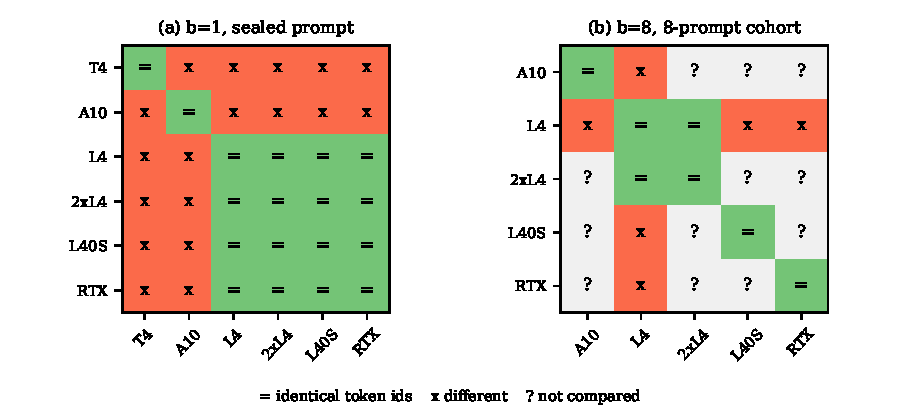
\includegraphics[width=0.85\linewidth]{figures/cross_gpu.pdf}
\caption{Token agreement between GPU types in r7. Each GPU is identical to itself at every host budget (diagonal). At $b=1$ the cards fall into three groups that follow the architecture: T4 (SM75), A10 (SM86), and SM89 plus Blackwell. At $b=8$ only the L4 pair was compared against every card; \emph{?} marks pairs we did not compare.}
\label{fig:crossgpu}
\end{figure}

\subsection{Throughput across GPUs}

\begin{figure}[htbp]
\centering
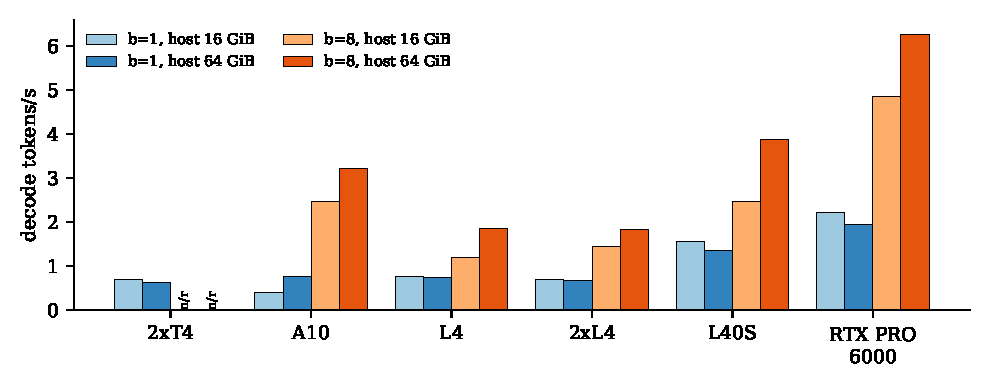
\includegraphics[width=\linewidth]{figures/r7_tps.pdf}
\caption{Decode tokens/s in r7 (aggregate over the batch at $b=8$). Next-use
eviction on both tiers. 2$\times$T4 ran batch 1 only (n/r).}
\label{fig:tps}
\end{figure}

\begin{table}[htbp]
\centering\small
\caption{r7 results. tok/s is aggregate at $b=8$. Host hit is over the last 32
decode steps. $B_\text{SSD}$ is the \texttt{fio} probe; a dagger marks a probe
that read the page cache.}
\label{tab:r7}
\begin{tabular}{lrrrrrrr}
\toprule
& \multicolumn{2}{c}{tok/s, $b=1$} & \multicolumn{2}{c}{tok/s, $b=8$} &
\multicolumn{2}{c}{host hit, $b=8$} & $B_\text{SSD}$ \\
GPU & 16\,GiB & 64\,GiB & 16\,GiB & 64\,GiB & 16 & 64 & GiB/s \\
\midrule
2$\times$T4 & 0.696 & 0.632 & --- & --- & --- & --- & 26.8$^\dagger$ \\
A10 & 0.411 & 0.756 & 2.470 & 3.230 & 0.433 & 0.853 & 1.43 \\
L4 & 0.766 & 0.732 & 1.204 & 1.866 & 0.439 & 0.848 & 4.52 \\
2$\times$L4 & 0.703 & 0.672 & 1.452 & 1.826 & 0.434 & 0.846 & 3.51 \\
L40S & 1.552 & 1.351 & 2.475 & 3.867 & 0.431 & 0.848 & 89$^\dagger$ \\
RTX PRO 6000 & 2.219 & 1.948 & 4.856 & 6.274 & 0.447 & 0.855 & 149$^\dagger$ \\
\bottomrule
\end{tabular}
\end{table}

Table~\ref{tab:r7} and Figure~\ref{fig:tps} give the r7 measurements. The RTX
PRO 6000 is fastest: 6.27 tokens/s aggregate at batch 8 with a 64\,GiB host
tier, about 3.4$\times$ the L4, and 2.2 tokens/s at batch 1. For reference, the
original Kaggle 2$\times$T4 anchor ran at about 0.21 tokens/s. Growing the host
tier from 16 to 64\,GiB roughly doubles the batch-8 host hit rate (0.43--0.45 to
0.85) and cuts cold reads per token from about 108 to about 29 on every GPU,
which raises batch-8 throughput by 1.3--1.6$\times$ (1.26$\times$ on 2$\times$L4;
Figure~\ref{fig:hosttier}). Per token, the A10 and RTX PRO 6000 are the cheapest
(about \$0.19 and \$0.22 per 1,000 tokens at list price; Figure~\ref{fig:cost}),
and 2$\times$L4 is the most expensive. These figures compare GPUs with each
other; they are not competitive with hosted inference (Section~\ref{sec:limits}).
A second GPU does not help: 2$\times$L4 is no faster than 1$\times$L4, which is
consistent with a single-stream engine whose bottleneck is the host-side read
and copy path, not GPU compute.

At batch 1 the 64\,GiB row is \emph{slower} than the 16\,GiB row on five of six
configurations, even though its host hit rate is higher (0.74 vs.\ 0.64). The
16\,GiB row runs first in each container, right after the store was staged
through the page cache, and a 64\,GiB pinned host tier leaves less RAM for the
operating system's page cache. Either could explain it; we have not tested
which, so we do not fit a batch-1 model and report this as an open anomaly. A repeat of r6's L4 batch-8 row in r7 gave 1.230 tokens/s against
1.204 for the same configuration later in the container (2\% apart), so
run-to-run noise at batch 8 is small compared with the effects above.

\begin{figure}[htbp]
\centering
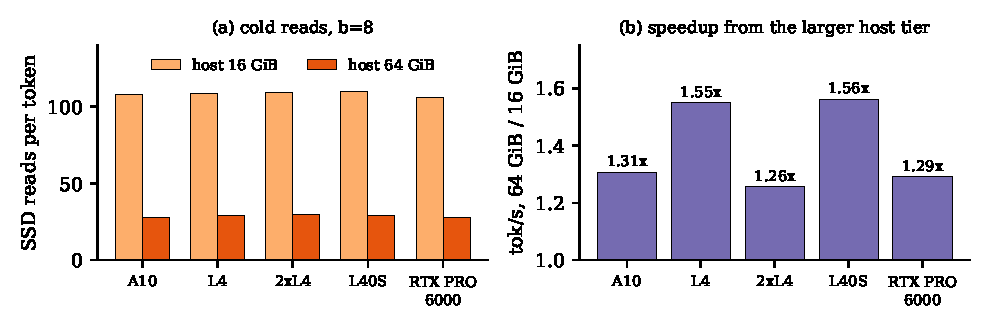
\includegraphics[width=\linewidth]{figures/host_tier.pdf}
\caption{Effect of the host tier at $b=8$ in r7. (a) A 64\,GiB tier cuts SSD reads per token about 3.7$\times$ on every GPU; the counts barely depend on the GPU because routing and cache policy are the same. (b) The resulting speedup is 1.26--1.56$\times$.}
\label{fig:hosttier}
\end{figure}

\begin{figure}[htbp]
\centering
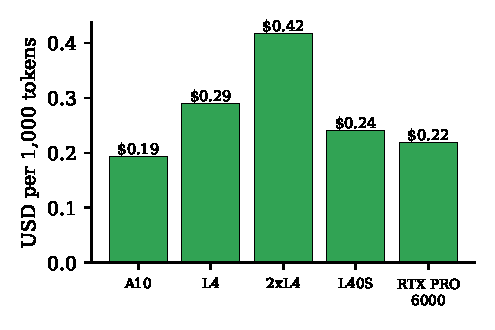
\includegraphics[width=0.5\linewidth]{figures/cost.pdf}
\caption{Cost per 1,000 generated tokens at $b=8$ with a 64\,GiB host tier, at Modal's all-in list rate (GPU, 8 CPU cores and reserved RAM). For scale, hosted APIs for the same model listed \$0.00018--0.00132 per 1,000 output tokens on 2026-11-20 \citep{openrouter2026dsv4}, so these rented-GPU costs are roughly 140--2,300$\times$ higher (Section~\ref{sec:limits}).}
\label{fig:cost}
\end{figure}

\subsection{Pre-registered predictions}

\begin{figure}[htbp]
\centering
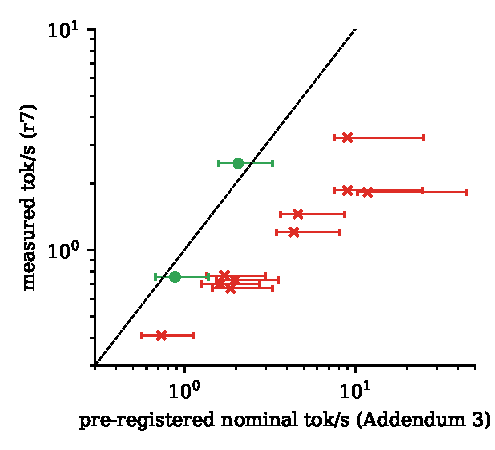
\includegraphics[width=0.55\linewidth]{figures/pred_vs_meas.pdf}
\caption{Addendum-3 predictions (nominal with registered range) against r7
measurements, for the 12 tokens/s rows that are testable. Circles: inside the
range; crosses: outside. The dashed line is $y=x$.}
\label{fig:pred}
\end{figure}

Figure~\ref{fig:pred} compares measured tokens/s with the Addendum-3
predictions for the three GPUs whose SSD bandwidth was measured. Of 12 testable
rows, 2 passed (A10 batch 1 at 64\,GiB, A10 batch 8 at 16\,GiB), 1 was weakened
and 9 were killed. On the L4 and 2$\times$L4 the engine ran 2.2--6.5$\times$
slower than the nominal prediction; the largest misses are at batch 8 with a
64\,GiB host tier, where the model predicted the cell to be bound by PCIe
copies. The same picture appeared in r5 (four L4 rows, all killed), before
the host-path fixes that made the engine about 1.8$\times$ faster between r5 and r6.

\begin{figure}[htbp]
\centering
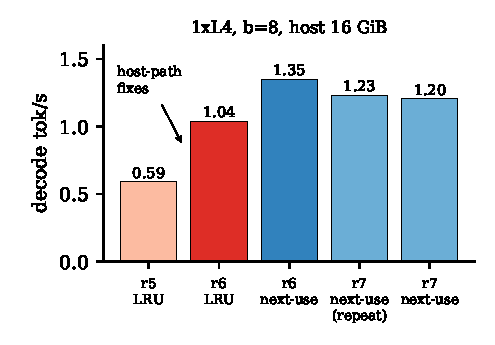
\includegraphics[width=0.5\linewidth]{figures/l4_progress.pdf}
\caption{Decode speed of the same L4 cell (b=8, 16\,GiB host tier) across runs. Host-path fixes between r5 and r6 gave 1.8$\times$ with the same reads per token; next-use eviction gave a further 1.30$\times$. The two r7 bars are the same configuration at the start and later in one container.}
\label{fig:progress}
\end{figure}

The stage profile from r5 shows why (Figure~\ref{fig:progress} shows how much
the later host-path fixes changed). At batch 8 with 64\,GiB, GPU copy time was
5.2\,s and GPU compute about 1\,s of a 640\,s row, while the host-side copy from
memory-mapped or read buffers into pinned memory took 262\,s of CPU time. The
engine read about 1.5\,GiB/s against 3.96\,GiB/s from \texttt{fio} on the same
disk. (The GPU copy timer may undercount: its event pool filled up during
this row.) The registered model assumed the host side was free. That assumption,
not the cache model, is what failed.

The cache predictions fared better. At 64\,GiB the host hit rate passed its
frozen band on every GPU. At 16\,GiB it was graded KILLED, but those frozen
rows predicted LRU, and r7 ran next-use. Under the prediction registered for
next-use (Addendum 5: 0.42, range 0.33--0.52) the r7 values of 0.43--0.45 at
batch 8 are inside the range on every GPU. At batch 1 the 16\,GiB rows were killed in the
other direction: 0.64 against an upper kill edge of 0.57, so the cache did
better than predicted. The simulator's unregistered next-use estimate for this
case was 0.67.

\subsection{Eviction and prefetch (run r6)}\label{sec:policy}

\begin{table}[htbp]
\centering\small
\caption{Addendum 5 predictions and r6 measurements (1$\times$L4, $b=8$, host
16\,GiB, last 32 decode steps). All four rows were byte-identical.}
\label{tab:r6}
\begin{tabular}{llrrl}
\toprule
id & metric & predicted [range] & measured & grade \\
\midrule
A1 & LRU host hit & 0.000 [0, 0.02] & 0.000 & PASS \\
A2 & next-use host hit & 0.42 [0.33, 0.52] & 0.439 & PASS \\
A3 & next-use cold reads per token & 115 [95, 140] & 108.4 & PASS \\
A4 & next-use VRAM hit & 0.12 [0.07, 0.18] & 0.125 & PASS \\
A5 & prev-step hints: host hit & 0.87 [0.72, 0.93] & 0.503 & \killed \\
A6 & hints: source reads vs.\ next-use & 1.00 [0.90, 1.20] & 1.266 & WEAKENED \\
A7 & hint hits per hint read & 0.77 [0.60, 0.92] & 0.311 & \killed \\
A8 & next-use / LRU tok/s & 1.27 [1.08, 1.50] & 1.300 & PASS \\
A9 & hints / next-use tok/s & 1.24 [1.05, 1.45] & 1.053 & PASS (edge) \\
\bottomrule
\end{tabular}
\end{table}

\begin{figure}[htbp]
\centering
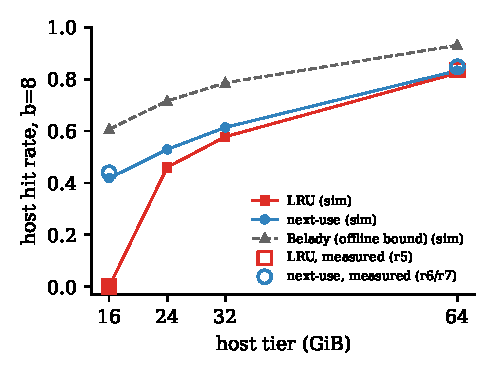
\includegraphics[width=0.55\linewidth]{figures/eviction_sizes.pdf}
\caption{Host hit rate at $b=8$ by host-tier size: trace-replay simulator (lines) and hardware (open markers). LRU collapses to 0 at 16\,GiB; next-use recovers 0.42 (measured 0.44); the offline Belady bound is 0.61. Above 32\,GiB the policies converge.}
\label{fig:eviction}
\end{figure}

\begin{figure}[htbp]
\centering
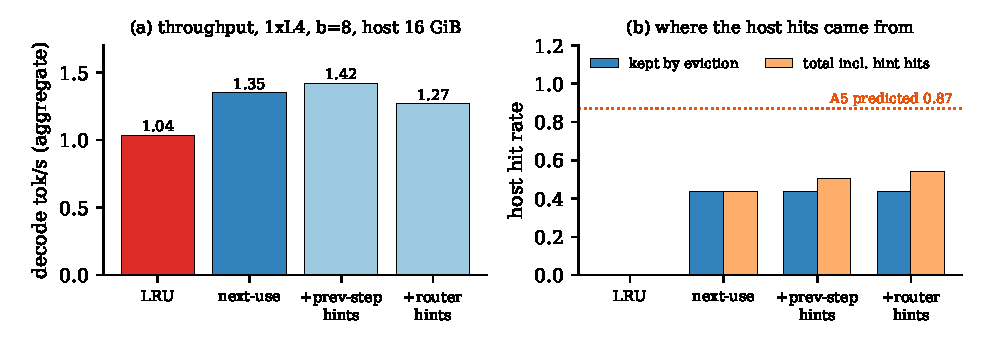
\includegraphics[width=\linewidth]{figures/r6_policies.pdf}
\caption{Run r6, one container, four placement policies with byte-identical outputs. (a) Throughput. (b) Host hit rate split into what eviction kept and what hints added. Hints added only 0.06--0.11 of hit rate against a predicted 0.87 total, at the cost of 27\% more reads.}
\label{fig:r6}
\end{figure}

Run r5 found the batch-8, 16\,GiB host tier at a hit rate of exactly 0 (0 of
49,463 lookups), because one decode step needs more records than the tier
holds and LRU evicts each one just before it is reused. A free trace-replay
simulator reproduced this (0.000) and the 64\,GiB rate (0.824 vs.\ 0.835
measured), and predicted that next-use eviction would recover 0.42 host hit
against an offline Belady bound of 0.61. Addendum 5 registered those numbers.
Table~\ref{tab:r6} and Figures~\ref{fig:eviction} and~\ref{fig:r6} show the outcome: every eviction prediction passed, and
next-use raised throughput 1.30$\times$ over LRU (1.348 vs.\ 1.037 tokens/s),
with cold reads per token down 44\%.

The hint predictions failed. Only 31\% of previous-step hint reads and 37\% of
router-hint reads were ever used; the router hints themselves had recall 0.77
and precision 0.77, but the hinted records were mostly ones that the cache
would not have kept anyway. The cause was a simulator bug, not an engine bug:
the simulator kept a finished hint available forever and admitted every hint.
With both fixed, it reproduces the measured row (host hit 0.522 vs.\ 0.503;
hint hits per read 0.28 vs.\ 0.31). This agrees with an earlier offline study
of six predictors on 50k routing events (empirical conditional, per-layer
conditional, hashed logistic, MLP, cross-layer and popularity), where every
predictor reached recall 0.05--0.52 at 8 candidates against a registered
0.65--0.80 and consumed 5--16$\times$ more bytes than it saved. We therefore
ship next-use eviction and leave hints off.

\subsection{A post-hoc throughput model}

After r7 we fitted a two-term model to the batch-8 rows:
\begin{equation}
T_\text{step} = t_\text{fixed}(\text{GPU}) + R_\text{cold} \cdot c_\text{read},
\end{equation}
where $R_\text{cold}$ is cold reads per step and $c_\text{read}$ the cost of one
12.75\,MiB record. Each GPU's 16/64\,GiB pair determines both terms (Figure~\ref{fig:tpsmodel}). The fitted
$t_\text{fixed}$ ranges from 3.41\,s/step (L4) to 1.14\,s/step (RTX PRO 6000) and
follows $t_\text{fixed} \approx 114\,\text{BW}^{-0.62}$ in the GPU's datasheet
memory bandwidth (GB/s). The fitted $c_\text{read}$ does \emph{not} follow the
\texttt{fio} bandwidth: the A10 has the slowest probe (1.43\,GiB/s) but reads
records about 3$\times$ faster than the L4, so the read cost is set by the
container and its page cache rather than by the raw disk. Predicting each GPU
from the other three (leave-one-GPU-out) gives a median absolute error of
14\% and a maximum of 56\% (L4 at 16\,GiB). This model was fitted after the
data and is not a pre-registration; we include it so that the next campaign
can register it.

\begin{figure}[htbp]
\centering
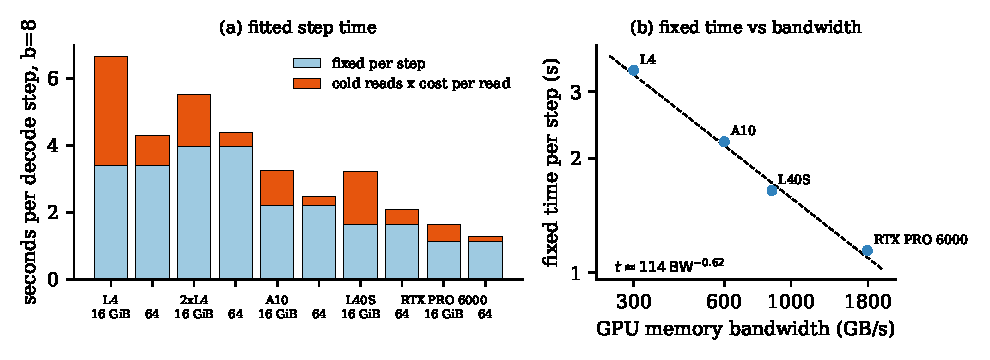
\includegraphics[width=\linewidth]{figures/tps_model.pdf}
\caption{Post-hoc step-time model at $b=8$. (a) Each bar splits a decode step into a fixed part and the cost of cold reads; the 64\,GiB rows (right of each pair) are mostly fixed time. (b) The fixed part falls with GPU memory bandwidth as a power law (2$\times$L4 omitted).}
\label{fig:tpsmodel}
\end{figure}

\section{Limitations}\label{sec:limits}

\begin{itemize}
\item \textbf{One model, one engine, small runs.} We evaluated DeepSeek-V4-Flash
only, with short generations (48 or 65 tokens) and a fixed 8-prompt cohort.
Our results say nothing about long-context behavior or other models. We have
not run competing systems ourselves.
\item \textbf{The reference is our own.} Exactness is relative to \dee{}'s
sealed reference path, not to DeepSeek's official kernels.
\item \textbf{Cross-GPU drift is not explained.} The near-tie hypothesis for
router flips is not verified, and at batch 8 the VRAM budget is confounded
with GPU model. The test that separates them is a run on the L40S or RTX PRO
6000 with the L4's 3,584\,MiB budget; if its tokens then match the L4, the
budget is innocent.
\item \textbf{Measurement caveats.} Modal does not let us drop the page cache
between rows in a container, three containers have no valid SSD bandwidth, and
the batch-1 16 vs.\ 64\,GiB anomaly is unexplained.
\item \textbf{Speed.} \dee{} is slower than recent systems that report results
on the same model and similar or larger hardware. Our profile points at the
host-side copy path as the main remaining cost.
\item \textbf{Cost and practicality.} Offloading trades throughput for memory,
and on rented hardware that trade is expensive. At the best measured setting
(batch 8, 64\,GiB host tier) a rented GPU container costs about \$0.19--0.42 per
1,000 generated tokens at list price (Figure~\ref{fig:cost}), i.e.\
\$190--420 per million. The same model, DeepSeek-V4-Flash-0731, is sold as a
hosted API by more than twenty providers. On 2026-11-20 their listed output
prices ranged from \$0.18 per million tokens (DeepInfra) to \$1.32 (Cloudflare
and others), with Cohere at \$0.28 \citep{openrouter2026dsv4}. Providers can
charge this because they keep the whole model in the memory of many GPUs and
batch hundreds of requests per forward pass. Our rented-GPU cost per token is
therefore roughly 140 to 2,300 times higher than hosted inference of the same
model. \dee{} is not a way to serve a model more cheaply than a
provider. It is useful where hosted inference is not an option or the GPU is
already paid for: a local or private deployment, offline use, a model too large
for the available VRAM, or research that needs to inspect and verify the
exact computation. On owned hardware the marginal cost is mostly electricity,
but at 0.7--2.2 tokens/s for a single stream the experience is still far from
interactive. The Phase-7 cost model predicted DEE could undercut dense,
fully resident serving at large batch; nothing in this campaign tested that
claim, and we do not make it.
\end{itemize}

\section{Conclusion}

Holding an MoE offloading engine to byte-identical outputs and to predictions
written before the experiment changed what we learned from it. Exactness held
on every GPU we ran, and an answer sealed three months earlier was reproduced token for token
on new infrastructure three months later. Most of our throughput predictions were wrong, which
located the real bottleneck (the host-side copy path) that a post-hoc model
would have absorbed into a fitted constant. Prefetch hints, which looked
promising in a simulator, failed on hardware for a reason we could then trace
to the simulator. Next-use eviction, predicted to fix a cache cliff, did so to
within 3\% of the registered speedup. We hope the frozen-prediction format,
the scorer and the exactness gate are useful to others evaluating offloading
systems, including faster ones than ours.

\paragraph{Availability.} Code, frozen predictions, addenda, scorecards and the
scorer are at \url{https://github.com/so-nerdyy/dee}. % TODO(Nivin): replace with a tagged release or commit hash once the repo is cleaned up.

\paragraph{Acknowledgments.} Much of the engineering, analysis and writing for
this project was done with the help of AI coding assistants (Claude, by
Anthropic). The author directed the work, made the design and evaluation
decisions, and takes responsibility for all content. Compute was paid for by the
author on Modal and Kaggle.

\bibliographystyle{plainnat}
\bibliography{refs}

\end{document}
